% ====================================================================
% graphite anode dQ/dV ICA theory document v7-08
% Chapter 1: equation-driven derivation arranged by Anode_Fit_v11_final.py
% ====================================================================
\documentclass[11pt,a4paper]{article}
\usepackage[margin=22mm]{geometry}
\usepackage{kotex}
\usepackage{fontspec}
\IfFontExistsTF{D2Coding}{\setmonofont{D2Coding}[Scale=MatchLowercase]}{\setmonofont{Latin Modern Mono}}
\usepackage{amsmath,amssymb,mathtools,bm}
\usepackage{booktabs,longtable,array}
\usepackage{enumitem}
\usepackage{amsthm}
\usepackage{tikz}
\usetikzlibrary{positioning,arrows.meta,calc}
\usepackage{hyperref}
\usepackage{fancyhdr}
\usepackage{lastpage}
\usepackage{setspace}
\setstretch{1.12}
\setlength{\parskip}{0.45em}
\setlength{\parindent}{0pt}
\setlength{\headheight}{14pt}
\setlength{\emergencystretch}{2em}
\hypersetup{colorlinks=true, linkcolor=blue, urlcolor=blue, citecolor=blue,
  pdftitle={Graphite anode dQ/dV ICA theory Chapter 1 v7-08}}
\pagestyle{fancy}\fancyhf{}
\lhead{Graphite anode $dQ/dV$ ICA theory — Ch.1 v7-08}
\rhead{\thepage/\pageref{LastPage}}
\renewcommand{\headrulewidth}{0.4pt}

\newtheorem*{keybox}{핵심}
\newtheorem*{verifybox}{검산}

\newcommand{\dd}{\mathrm{d}}
\newcommand{\eq}{\mathrm{eq}}
\newcommand{\app}{\mathrm{app}}
\newcommand{\bg}{\mathrm{bg}}
\newcommand{\eff}{\mathrm{eff}}
\newcommand{\hys}{\mathrm{hys}}
\newcommand{\cell}{\mathrm{cell}}
\newcommand{\work}{\mathrm{work}}
\newcommand{\lag}{\mathrm{lagged}}
\newcommand{\dis}{\mathrm{dis}}
\newcommand{\chg}{\mathrm{chg}}
\newcommand{\artanh}{\operatorname{artanh}}
\renewcommand{\theequation}{1.\arabic{equation}}
\renewcommand{\thesection}{N\arabic{section}}

\title{\textbf{\LARGE Chapter 1}\\[0.35em]\Large 흑연 음극 $dQ/dV$ ICA 이론: v11 코드 진행순서형 수식 전개}
\author{}
\date{}

\begin{document}
\maketitle
\tableofcontents
\newpage
\setcounter{section}{-1}

본 장의 목적은 \texttt{GraphiteAnodeDischargeDQDV.curve}가 실험 조건을 받아
\texttt{dqdv}로 내려보낸 뒤, \texttt{dqdv}가 한 곡선을 계산하는 순서 그대로 물리식을 닫는 것이다.
따라서 절 순서는 \texttt{v11\_flowchart.md}의 N0--N9를 따른다. 본문에서 새로 도입되는 기호는
코드 식별자와 같은 역할을 갖는다. 방향 부호는
\begin{equation}
\sigma_d=\begin{cases}
+1,&\text{방전, discharge},\\
-1,&\text{충전, charge},
\end{cases}
\qquad |I|\ge0,\qquad q=\frac{Q}{Q_{\cell}}.
\label{eq:sigmadef}
\end{equation}
본 장이 반환할 관측량은 방향 정렬된 양의 ICA 크기
\begin{equation}
\frac{\dd Q}{\dd V}\equiv \frac{\dd Q}{\dd V_{\app}}
\label{eq:targetdqdv}
\end{equation}
이며, 실제 독립축은 먼저 내부 음극 전위 $V_n$로 환산된다.

% ====================================================================
\section{N0. 실험조건에서 모델 입력으로}\label{sec:N0}
% ====================================================================
\texttt{curve}는 방향 라벨, C-rate, 셀 용량, 온도, 선택적 전류 크기를 코드 코어의 입력으로 바꾼다.
방향 라벨은 식~\eqref{eq:sigmadef}의 $\sigma_d$로만 남고, 전류 크기는
\begin{equation}
|I|=\begin{cases}
I_{\mathrm{abs}},& I_{\mathrm{abs}}\ \text{가 주어질 때},\\
c_{\mathrm{rate}}\,Q_{\cell},& I_{\mathrm{abs}}\ \text{가 없을 때}.
\end{cases}
\label{eq:Iabs}
\end{equation}
이 변환은 새 물리가 아니라 단위 사상이다. 물리 계산의 독립 입력은
\begin{equation}
\mathcal D=\{V_{\app},\,T,\,|I|,\,Q_{\cell},\,\sigma_d\}
\quad\Longrightarrow\quad
\texttt{dqdv}(V_{\app},T,|I|,Q_{\cell},s=\sigma_d)
\label{eq:inputset}
\end{equation}
이다.

\begin{figure}[t]
\centering
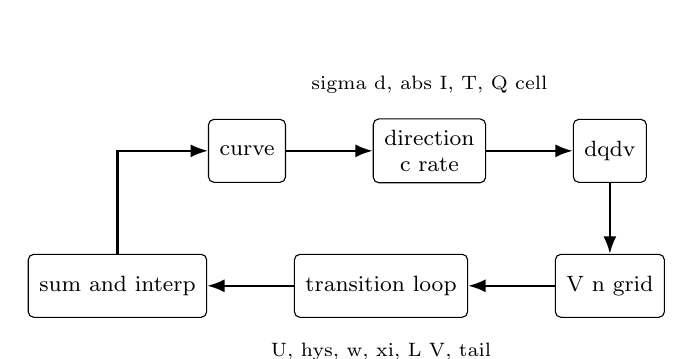
\begin{tikzpicture}[node distance=9mm and 11mm,
box/.style={draw,rounded corners=2pt,minimum height=8mm,align=center,font=\footnotesize,inner sep=4pt},
arr/.style={-{Latex[length=2.2mm]},thick}]
\node[box] (curve) {curve};
\node[box,right=of curve] (map) {direction\\c rate};
\node[box,right=of map] (core) {dqdv};
\node[box,below=of core] (vn) {V n grid};
\node[box,left=of vn] (loop) {transition loop};
\node[box,left=of loop] (sum) {sum and interp};
\draw[arr] (curve) -- (map);
\draw[arr] (map) -- (core);
\draw[arr] (core) -- (vn);
\draw[arr] (vn) -- (loop);
\draw[arr] (loop) -- (sum);
\draw[arr] (sum) |- (curve);
\node[font=\scriptsize,above=2mm of map] {sigma d, abs I, T, Q cell};
\node[font=\scriptsize,below=2mm of loop] {U, hys, w, xi, L V, tail};
\end{tikzpicture}
\caption{코드 진행의 최상위 사상. 그림 안의 모든 텍스트는 ASCII로만 두었다. 이 그림은 식~\eqref{eq:inputset}에서 시작해 N1--N9가 어떤 순서로 필요한지 보여준다.}
\label{fig:codeflow}
\end{figure}

그림~\ref{fig:codeflow}의 화살표가 본 장의 순서다. 다음 절은 관측 전위 $V_{\app}$를 내부 전위 $V_n$으로 바꾸는 첫 계산을 닫는다.

% ====================================================================
\section{N1. 분극과 작업격자}\label{sec:N1}
% ====================================================================
코어의 첫 물리식은 분극 제거다. v11의 부호는
\begin{equation}
\boxed{\;V_n=V_{\app}-\sigma_d |I|R_n\;}
\label{eq:polarization}
\end{equation}
이다. 방전에서 $\sigma_d=+1$이므로 관측 전위에서 $|I|R_n$을 빼 내부 전위를 얻고, 충전에서 $\sigma_d=-1$이므로 같은 크기를 더한다. 이 부호는 방전, 즉 de-lithiation과 oxidation에서 측정 전위 $V_{\app}$가 내부 평형 음극 전위보다 높다는 양의 anodic 과전압 $\eta=V_{\app}-V_n>0$을 코드의 내부 전위 좌표로 옮긴 결과다.

작업격자는 꼬리의 지지 영역을 잃지 않도록 $V_n$ 범위보다 넓게 잡힌다.
\begin{align}
v_{\mathrm{lo}}&=\min V_n,\qquad v_{\mathrm{hi}}=\max V_n,\qquad
v_{\mathrm{span}}=\max(v_{\mathrm{hi}}-v_{\mathrm{lo}},v_{\mathrm{span,floor}}),\label{eq:vspan}\\
n_{\work}&=\max(n_{\work,\min},\,2\,N_V),\label{eq:nwork}\\
V_{\work}&=\operatorname{linspace}\!\left(v_{\mathrm{lo}}-g_{\mathrm{lo}}v_{\mathrm{span}},\,
v_{\mathrm{hi}}+g_{\mathrm{hi}}v_{\mathrm{span}},\,n_{\work}\right),\label{eq:vwork}\\
\Delta V_{\work}&=V_{\work,k+1}-V_{\work,k}.
\label{eq:gridstep}
\end{align}
온도가 배열이면 $V_n$ 순서로 정렬해 $V_{\work}$ 위에 보간하고, 스칼라면 상수 배열로 복제한다.
\begin{equation}
T_{\work}(V)=
\begin{cases}
\operatorname{interp}(V;V_n,T),&T\ \text{가 배열일 때},\\
T\,\mathbf 1,&T\ \text{가 스칼라일 때},
\end{cases}
\qquad
T_{\mathrm{rep}}=\operatorname{mean}(T_{\work}).
\label{eq:Twork}
\end{equation}
배경은 전이 반복 전에 초기화된다.
\begin{equation}
dqdv_{\work}^{(0)}(V_{\work})=
\begin{cases}
C_{\bg}(V_{\work}),&C_{\bg}\ \text{가 callable일 때},\\
C_{\bg}\,\mathbf 1,&C_{\bg}\ \text{가 상수일 때}.
\end{cases}
\label{eq:Cbginit}
\end{equation}
이제 전이 $j$마다 평형 중심을 계산한다.

% ====================================================================
\section{N2. 평형 중심 $U_j(T)$}\label{sec:N2}
% ====================================================================
전이 중심은 Gibbs 자유에너지에서 온다. 삽입 반응의 몰 자유에너지를 전위로 환산하면
\begin{equation}
\Delta G_j(T)=\Delta H_{\mathrm{rxn},j}-T\Delta S_{\mathrm{rxn},j},
\qquad
\Delta G_j=-F\,U_j.
\label{eq:gibbsU}
\end{equation}
따라서 코드의 \texttt{func\_U\_j}와 같은 식은
\begin{equation}
\boxed{\;U_j(T)=\frac{-\Delta H_{\mathrm{rxn},j}+T\Delta S_{\mathrm{rxn},j}}{F}\;}
\label{eq:UjT}
\end{equation}
이다. 전이 사전에 \texttt{dH\_rxn}과 \texttt{dS\_rxn}이 있으면 식~\eqref{eq:UjT}를 쓰고, 없으면 직접 주어진 \texttt{U}가 중심이다.
\begin{equation}
U_j=
\begin{cases}
\texttt{func\_U\_j}(T_{\work},\texttt{dH\_rxn}_j,\texttt{dS\_rxn}_j),&
\{\texttt{dH\_rxn},\texttt{dS\_rxn}\}\subset tr_j,\\
\texttt{U}_j,&\text{otherwise}.
\end{cases}
\label{eq:Udispatch}
\end{equation}
이 중심은 아직 방향을 모른다. 방향은 히스테리시스 분기 중심에서만 들어간다.

% ====================================================================
\section{N3. 히스테리시스 분기}\label{sec:N3}
% ====================================================================
정규용액 상호작용이 충분히 강하면 균일 등온선은 spinodal을 갖는다. 보편형은
\begin{equation}
g_j(\xi)=g_j^0+RT\{\xi\ln\xi+(1-\xi)\ln(1-\xi)\}
\,+\,\Omega_j\xi(1-\xi)
\label{eq:gxi}
\end{equation}
이고,
\begin{equation}
g_j''(\xi)=\frac{RT}{\xi(1-\xi)}-2\Omega_j.
\label{eq:gpp}
\end{equation}
spinodal은 $g_j''=0$이므로
\begin{align}
\frac{RT}{\xi(1-\xi)}&=2\Omega_j,\label{eq:spinodalstep1}\\
\xi(1-\xi)&=\frac{RT}{2\Omega_j},\label{eq:spinodalstep2}\\
\left(\xi-\frac12\right)^2
&=\frac14-\frac{RT}{2\Omega_j}.
\label{eq:spinodalstep3}
\end{align}
따라서
\begin{equation}
\xi_{s,j}^{\pm}=\frac12\pm\frac12 u_j,\qquad
u_j=\sqrt{1-\frac{2RT}{\Omega_j}},\qquad \Omega_j>2RT.
\label{eq:spinodal}
\end{equation}
두 spinodal 전위의 차를 대칭 중심 $U_j$ 주위의 gap으로 쓰면 v11의 \texttt{func\_dU\_hys}가 된다.
\begin{equation}
\boxed{\;
\Delta U_j^{\hys}(T,\Omega_j)=
\begin{cases}
0,&\Omega_j\le2RT,\\[2pt]
\dfrac{2}{F}\left[\Omega_j u_j-2RT\,\artanh u_j\right],&\Omega_j>2RT.
\end{cases}
\;}
\label{eq:dUhys}
\end{equation}
부분 cycle 인자 $h_\eta$와 축소 인자 $\gamma_j$를 곱하면 코드의 분기 중심은
\begin{equation}
\boxed{\;U_j^d=U_j+\frac12\,\sigma_d\,h_\eta\,\gamma_j\,\Delta U_j^{\hys}\;}
\label{eq:Ubranch}
\end{equation}
이다. v11 구현은 \texttt{func\_U\_branch(T\_rep,0,Omega,gamma,sigma\_d,h\_eta)}로 shift를 만들고 이를 배열 $U_j(T_{\work})$에 더한다.
\begin{equation}
\mathrm{center}_j(V_{\work})=
\begin{cases}
U_j(V_{\work})+\texttt{func\_U\_branch}(T_{\mathrm{rep}},0,\Omega_j,\gamma_j,\sigma_d,h_\eta),
&\gamma_j\ne0,\ \Omega_j>0,\\
U_j(V_{\work}),&\text{otherwise}.
\end{cases}
\label{eq:centerdispatch}
\end{equation}

\begin{figure}[t]
\centering
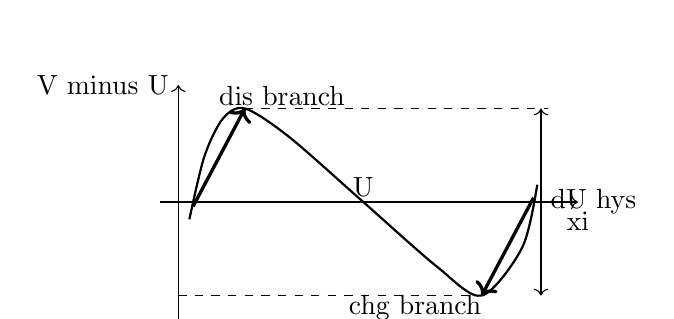
\begin{tikzpicture}[x=4.7cm,y=1.1cm]
\draw[->] (-0.05,0) -- (1.08,0) node[below] {xi};
\draw[->] (0,-1.35) -- (0,1.35) node[left] {V minus U};
\draw[thick] plot[smooth] coordinates {(0.03,-0.2) (0.07,0.52) (0.12,0.96) (0.18,1.08) (0.30,0.75) (0.50,0) (0.70,-0.75) (0.82,-1.08) (0.93,-0.52) (0.97,0.2)};
\draw[dashed] (0.18,1.08) -- (1.0,1.08);
\draw[dashed] (0.0,-1.08) -- (0.82,-1.08);
\draw[<->] (0.98,-1.08) -- (0.98,1.08) node[pos=0.5,right] {dU hys};
\draw[->,very thick] (0.04,-0.05) -- (0.18,1.08);
\draw[->,very thick] (0.96,0.05) -- (0.82,-1.08);
\node at (0.28,1.22) {dis branch};
\node at (0.64,-1.22) {chg branch};
\node at (0.50,0.17) {U};
\end{tikzpicture}
\caption{히스테리시스 분기 중심의 대칭 구조. 본문은 식~\eqref{eq:dUhys}와 식~\eqref{eq:Ubranch}를 이 그림의 두 수직 이동으로 사용한다.}
\label{fig:hysbranch}
\end{figure}

그림~\ref{fig:hysbranch}의 방전과 충전 중심 이동은 항상 반대다. 다음 절에서는 이 중심 주위의 폭을 정한다.

% ====================================================================
\section{N4. 폭 $w$와 유효폭}\label{sec:N4}
% ====================================================================
폭은 전위 변화가 점유율 변화를 얼마나 넓게 펼치는지를 정한다. 같은 총 전이 용량이라도 폭이 작으면 peak는 높고 좁아지며, 폭이 크면 낮고 넓어진다.

이상 격자기체의 정지점은 폭
\begin{equation}
\boxed{\;w_j(T)=\frac{n_jRT}{F}\;}
\label{eq:w}
\end{equation}
를 갖는다. v11의 \texttt{\_n\_factor}는 \texttt{n}이 있으면 그대로 쓰고, \texttt{w}가 있으면
\begin{equation}
n_j=\frac{w_jF}{RT}
\label{eq:nfromw}
\end{equation}
로 역산하며, 둘 다 없으면 $n_j=1$이다.
\begin{equation}
n_j(T)=
\begin{cases}
\texttt{n}_j,&\texttt{n}_j\ne\varnothing,\\
\texttt{w}_jF/(RT),&\texttt{w}_j\ne\varnothing,\\
1,&\text{otherwise}.
\end{cases}
\label{eq:nfactor}
\end{equation}
상호작용 좁힘은 OCV 곡선의 국소 기울기를 같은 logistic 폭으로 치환하는 단계다. 먼저 정규용액 OCV를 점유율의 함수로 쓰면
\begin{align}
V_j(\xi;T,\Omega_j)
&=U_j(T)+\frac{RT}{F}\ln\frac{\xi}{1-\xi}
+\frac{\Omega_j}{F}(1-2\xi),\label{eq:ocvregular}\\
\Delta U_{j,\mathrm{signed}}^{\hys}(\xi)
&=V_{j,\chg}(\xi)-V_{j,\dis}(\xi),\qquad
\Delta U_j^{\hys}=\left|\Delta U_{j,\mathrm{signed}}^{\hys}\right|,\label{eq:hysocvstep}\\
\frac{\dd V_j}{\dd \xi}
&=\frac{RT}{F}\left(\frac1{\xi}+\frac1{1-\xi}\right)-\frac{2\Omega_j}{F},\qquad
w_j^{\eff}=\frac14\left.\frac{\dd V_j}{\dd \xi}\right|_{\xi=1/2}.
\label{eq:weffbridge}
\end{align}
현재 부호 규약에서는 방전 branch가 충전 branch보다 높은 전위에 놓이므로 식~\eqref{eq:hysocvstep}의 signed 차이는 음수일 수 있다. 코드의 \texttt{func\_dU\_hys}와 식~\eqref{eq:dUhys}는 이 차이의 비음수 크기를 만들고, 실제 방전과 충전의 위상은 식~\eqref{eq:Ubranch}의 $\sigma_d$가 부여한다. 따라서 중심 기울기 일치에서
\begin{equation}
w_j^{\eff}(T,\Omega_j)=\frac{RT}{F}\left(1-\frac{\Omega_j}{2RT}\right)
\label{eq:weffraw}
\end{equation}
가 나오고, 구현은 폭 0에 의한 발산을 막기 위해
\begin{equation}
\boxed{\;\texttt{func\_w\_eff}=\max\!\left[
\frac{RT}{F}\left(1-\frac{\Omega_j}{2RT}\right),\,
f_{\mathrm{floor}}\frac{RT}{F}\right]\;}
\label{eq:weff}
\end{equation}
를 쓴다. 실제 dispatch는
\begin{equation}
w_j=
\begin{cases}
\texttt{func\_w\_eff}(T,\Omega_j,f_{\mathrm{floor}}),
&\texttt{use\_w\_eff=True},\ \Omega_j\ne\varnothing,\ \texttt{w}_j=\varnothing,\\
\texttt{func\_w}(T,n_j),&\text{otherwise}.
\end{cases}
\label{eq:wdispatch}
\end{equation}
이다.

% ====================================================================
\section{N5. 평형 점유 $\xi_{\eq}$}\label{sec:N5}
% ====================================================================
점유율은 전위축 위의 peak 위치를 전하축 위의 진행률로 바꾸는 내부 상태 변수다. \texttt{dqdv}에서는 히스테리시스 분기 중심 $U_j^d$를 써서 현재 branch 위의 순간 평형 점유를 계산한다.

정방향과 역방향 속도의 detailed balance는
\begin{equation}
\frac{r_j^+}{r_j^-}=\exp\!\left(\frac{\sigma_d(V_n-U_j^d)}{w_j}\right)
\label{eq:db}
\end{equation}
를 요구한다. 정지점에서 $r_j^+(1-\xi_{\eq,j})=r_j^-\xi_{\eq,j}$이므로
\begin{equation}
\frac{\xi_{\eq,j}}{1-\xi_{\eq,j}}
=\exp\!\left(\frac{\sigma_d(V_n-U_j^d)}{w_j}\right).
\label{eq:logit}
\end{equation}
따라서 v11의 \texttt{func\_ksi\_eq}는
\begin{equation}
\boxed{\;\xi_{\eq,j}(V,T,\sigma_d)
=\frac{1}{1+\exp[-z_j]},\qquad
z_j=\frac{\sigma_d(V-U_j^d)}{w_j}\;}
\label{eq:xieq}
\end{equation}
이다. 구현은 $z_j\ge0$과 $z_j<0$를 나누어 overflow를 피하지만 수학식은 식~\eqref{eq:xieq} 하나다.

\begin{figure}[t]
\centering
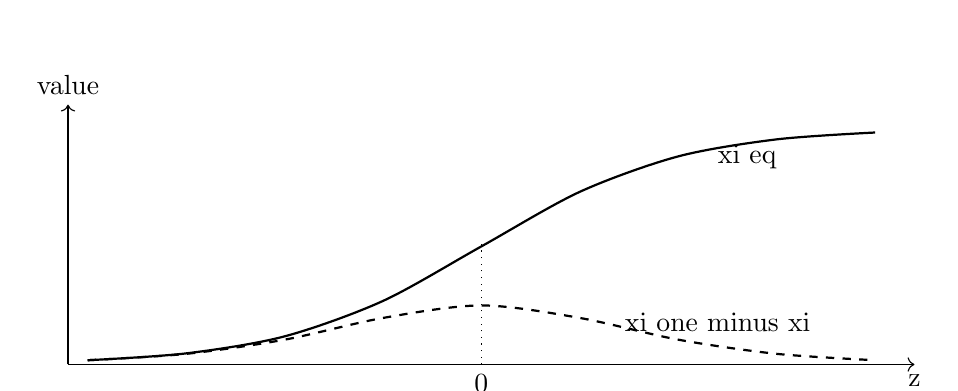
\begin{tikzpicture}[x=1.25cm,y=3.0cm]
\draw[->] (-4.2,0) -- (4.4,0) node[below] {z};
\draw[->] (-4.2,0) -- (-4.2,1.1) node[above] {value};
\draw[thick] plot[smooth] coordinates {(-4,0.018) (-3,0.047) (-2,0.119) (-1,0.269) (0,0.5) (1,0.731) (2,0.881) (3,0.953) (4,0.982)};
\draw[thick,dashed] plot[smooth] coordinates {(-4,0.018) (-3,0.045) (-2,0.105) (-1,0.197) (0,0.25) (1,0.197) (2,0.105) (3,0.045) (4,0.018)};
\draw[dotted] (0,0) -- (0,0.52);
\node at (2.7,0.88) {xi eq};
\node at (2.4,0.18) {xi one minus xi};
\node[below] at (0,0) {0};
\end{tikzpicture}
\caption{식~\eqref{eq:xieq}의 logistic과 그 미분 핵 $\xi_{\eq}(1-\xi_{\eq})$. N6의 평형 peak는 이 dashed curve를 $w_j$로 나눈다.}
\label{fig:logisticpeak}
\end{figure}

그림~\ref{fig:logisticpeak}의 중심 $z=0$은 $V=U_j^d$다. 이 점에서 평형 peak가 최대가 된다.

% ====================================================================
\section{N6. 평형 peak와 \texttt{equilibrium()}}\label{sec:N6}
% ====================================================================
평형 peak는 유한 전류 꼬리를 붙이기 전의 기준 모양이다. 이 기준선은 \texttt{equilibrium()}에서 직접 쓰이며, 히스테리시스 branch midpoint가 아니라 hysteresis-free OCV baseline에서 정해진다.

\begin{align}
V_{\eq,j}(\xi;T)&=U_j(T)+w_j(T)\ln\frac{\xi}{1-\xi},\label{eq:Veqbaseline}\\
V_{\app}&=V_{\eq,j}(\xi_{\eq,j})
\qquad (|I|=0,\ R_n=0,\ \gamma_j=0).\label{eq:VappVeqxieq}
\end{align}
따라서 \texttt{equilibrium()}의 $\xi_{\eq,j}$는 $U_j^d$에 고정된 branch 점유가 아니라 식~\eqref{eq:Veqbaseline}의 $V_{\eq}$에서 결정된다. 이를 풀면 식~\eqref{eq:xieq}의 $\gamma_j=0$ 기준식이 된다. 식~\eqref{eq:xieq}를 미분하면
\begin{align}
\frac{\dd \xi_{\eq,j}}{\dd z_j}
&=\xi_{\eq,j}(1-\xi_{\eq,j}),\label{eq:dxidz}\\
\frac{\dd z_j}{\dd V}
&=\frac{\sigma_d}{w_j},\label{eq:dzdV}\\
\frac{\dd \xi_{\eq,j}}{\dd V}
&=\frac{\sigma_d\,\xi_{\eq,j}(1-\xi_{\eq,j})}{w_j}.
\label{eq:dxidVsig}
\end{align}
ICA peak는 방향 정렬된 양의 크기이므로 코드의 평형 peak shape는 절댓값을 취한 것과 같다.
\begin{equation}
\boxed{\;\texttt{peak\_shape}_{j,\eq}
=\frac{\xi_{\eq,j}(1-\xi_{\eq,j})}{w_j}
=\left|\frac{\dd \xi_{\eq,j}}{\dd V}\right|\;}
\label{eq:eqpeakshape}
\end{equation}
전이 용량 $Q_j$를 곱하고 배경을 더하면 \texttt{equilibrium(V\_n,T)}가 된다.
\begin{equation}
\boxed{\;\mathrm{equilibrium}(V_n,T)
=C_{\bg}(V_n)+\sum_{j=1}^{N_p}Q_j\frac{\xi_{\eq,j}(1-\xi_{\eq,j})}{w_j}\;}
\label{eq:equilibrium}
\end{equation}
이는 $|I|\to0$, $\gamma_j=0$ 또는 분기를 쓰지 않는 한계, $L_{V,j}$가 sub-grid인 한계에서 \texttt{dqdv}가 회수하는 식이다.
\begin{equation}
|I|\to0\quad\Longrightarrow\quad
L_{q,j}\propto |I|\to0,\qquad
\texttt{peak\_shape}_j\to\texttt{peak\_shape}_{j,\eq}.
\label{eq:equilimit}
\end{equation}
다음 절은 $L_{V,j}$가 sub-grid보다 클 때 peak가 왜 뒤로 끌리는지 정한다.

% ====================================================================
\section{N7. 동역학 꼬리 길이 $L_V$}\label{sec:N7}
% ====================================================================
유한 전류에서는 점유율이 순간 평형값을 즉시 따라가지 못한다. 이 절의 목적은 시간 지연 길이 $L_q$를 전압축 길이 $L_V$로 바꾸어, 다음 절의 causal memory kernel이 사용할 단일 길이 척도를 만드는 것이다.

완화식은
\begin{equation}
\frac{\dd \xi_j}{\dd t}=k_j(\xi_{\eq,j}-\xi_j)
\label{eq:relax}
\end{equation}
이고, $\dd q/\dd t=|I|/Q_{\cell}$이므로
\begin{equation}
\frac{\dd \xi_j}{\dd q}=\frac{Q_{\cell}k_j}{|I|}(\xi_{\eq,j}-\xi_j),
\qquad
L_{q,j}=\frac{|I|}{Q_{\cell}k_j}.
\label{eq:Lqdef}
\end{equation}
Eyring--Butler--Volmer 형식에서
\begin{equation}
k_j=\frac{k_BT}{h}
\exp\!\left[-\frac{\Delta H_{a,j}^{\eff}-T\Delta S_{a,j}-\chi_d A_j}{RT}\right]
\left(1+e^{-A_j/RT}\right)
\label{eq:kuniv}
\end{equation}
이므로 v11의 \texttt{func\_L\_q}는
\begin{align}
L_{q,j}
&=\frac{|I|}{Q_{\cell}k_j},\label{eq:Lqfromk}\\
\ln L_{q,j}
&=\ln\frac{|I|h}{Q_{\cell}k_BT}
+\frac{\Delta H_{a,j}^{\eff}-T\Delta S_{a,j}-\chi_d A_j}{RT}
-\ln\!\left(1+e^{-A_j/RT}\right)
\label{eq:lnLqintermediate}
\end{align}
를 거쳐
\begin{equation}
\boxed{\;
L_{q,j}=
\frac{|I|h}{Q_{\cell}k_BT}\,
\frac{\exp[(\Delta H_{a,j}^{\eff}-T\Delta S_{a,j}-\chi_d A_j)/RT]}
{1+e^{-A_j/RT}}\;}
\label{eq:Lq}
\end{equation}
와 같다. 코드에서 \texttt{func\_L\_q}의 인자 \texttt{x}가 바로 $\chi_d$다.

방향별 전달계수는
\begin{equation}
\boxed{\;\chi_d=
\begin{cases}
\chi,&\sigma_d\ge0,\\
1-\chi,&\sigma_d<0,
\end{cases}
\qquad
\Delta H_{a,j}^{\eff}=\Delta H_{a,j}-\chi_d\Omega_j\;}
\label{eq:chidHeff}
\end{equation}
이다. 꼬리 컷 affinity는 정점 이후 $\xi_{\eq}$ 원천이 작아진 지점을 대표하는 양으로 코드에서
\begin{equation}
A_j=\min\{z_{\mathrm{cut}}\,n_jRT,\ A_{\mathrm{cap,RT}}\,RT\}
\label{eq:Acut}
\end{equation}
로 만든다. $A_j$는 크기이며 방향 부호를 갖지 않는다. 방향은 식~\eqref{eq:chidHeff}의 $\chi_d$와 N8의 격자 진행방향이 받는다.

전압축 길이는
\begin{equation}
\boxed{\;L_{V,j}=|dV/dq|_{q_a}\,L_{q,j}\;}
\label{eq:LV}
\end{equation}
이며, v11에서는 전이 사전의 \texttt{dVdq\_qa}가 $|dV/dq|_{q_a}$ 역할을 한다. 전이 사전에 직접 \texttt{L\_V}가 있으면 식~\eqref{eq:Lq}--\eqref{eq:LV}를 우회하고 그 값을 쓴다.

전위가 높아지면 affinity가 커지고 장벽은 낮아진다. 활성화 지배에서
\begin{equation}
\frac{\partial\ln L_{q,j}}{\partial V}
=-\frac{\chi_d}{RT}\frac{\partial A_j}{\partial V}<0
\label{eq:dlnLdV}
\end{equation}
이다. 이 부호가 ``$V$가 올라가면 꼬리가 짧아진다''는 체크리스트 항목이다.

% ====================================================================
\section{N8. 인과 기억 꼬리와 충전 격자 역전}\label{sec:N8}
% ====================================================================
꼬리는 평형 peak를 새로 만드는 항이 아니라 이전 전위에서 남은 점유 지연을 현재 전위로 운반하는 항이다. 따라서 핵심은 kernel의 모양보다 어느 방향이 시간적으로 과거인지 정하는 데 있다.

지연 $r_j=\xi_{\eq,j}-\xi_j$는
\begin{equation}
\frac{\dd r_j}{\dd q}=\frac{\dd \xi_{\eq,j}}{\dd q}-\frac{r_j}{L_{q,j}}
\label{eq:rodeo}
\end{equation}
를 만족한다. $L_{q,j}$가 국소 상수이면 적분인자로
\begin{equation}
r_j(q)=r_j(q_0)e^{-(q-q_0)/L_{q,j}}
\,+\,\int_{q_0}^{q}
e^{-(q-q')/L_{q,j}}\frac{\dd\xi_{\eq,j}}{\dd q'}\,\dd q'
\label{eq:memory}
\end{equation}
가 된다. 전압 균일격자에서는 이 합성곱을 1차 causal low-pass로 구현한다.
\begin{align}
\alpha_j&=\exp(-\Delta V_{\work}/L_{V,j}),\label{eq:alpha}\\
\xi_{\lag,k}&=(1-\alpha_j)\xi_{\eq,k}+\alpha_j\xi_{\lag,k-1}.
\label{eq:lowpass}
\end{align}
v11의 \texttt{\_causal\_lowpass}는 식~\eqref{eq:lowpass}를 \texttt{lfilter} 또는 명시 loop로 계산한다.

중요한 것은 ``과거''의 방향이다. 방전은 $V_{\work}$ 오름차순이 진행방향이므로 그대로 필터링한다.
\begin{equation}
\sigma_d\ge0:\qquad
\xi_{\lag}=\texttt{\_causal\_lowpass}(\xi_{\eq},\Delta V_{\work},L_V).
\label{eq:dislowpass}
\end{equation}
충전은 진행방향이 $V$ 감소이므로 배열을 뒤집어 필터링한 뒤 다시 뒤집는다.
\begin{equation}
\boxed{\;\sigma_d<0:\qquad
\xi_{\lag}=
\texttt{\_causal\_lowpass}(\xi_{\eq}[::-1],\Delta V_{\work},L_V)[::-1]\;}
\label{eq:chargelowpass}
\end{equation}
따라서 동역학 peak shape는
\begin{equation}
\boxed{\;\texttt{peak\_shape}_j
=\frac{\xi_{\eq,j}-\xi_{\lag,j}}{L_{V,j}}\;}
\label{eq:tailpeak}
\end{equation}
이다. $L_{V,j}$가 충분히 작거나 유한하지 않으면 식~\eqref{eq:eqpeakshape}를 쓰는 분기로 돌아간다.
\begin{equation}
L_{V,j}<\texttt{min\_lag\_grid\_steps}\,\Delta V_{\work}
\quad\Longrightarrow\quad
\texttt{peak\_shape}_j=\frac{\xi_{\eq,j}(1-\xi_{\eq,j})}{w_j}.
\label{eq:minlagbranch}
\end{equation}

\begin{figure}[t]
\centering
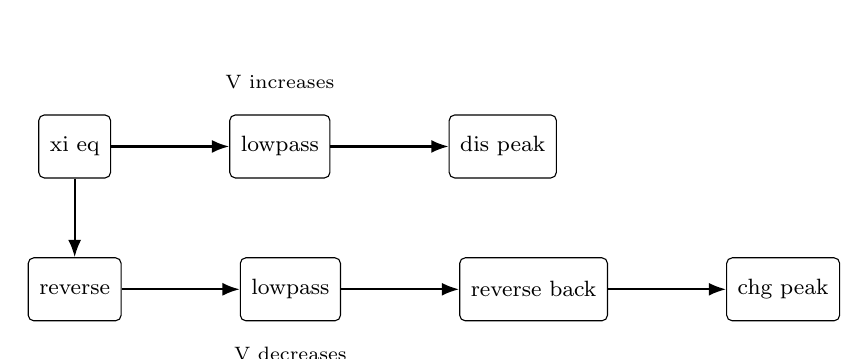
\begin{tikzpicture}[node distance=10mm and 15mm,
box/.style={draw,rounded corners=2pt,minimum height=8mm,align=center,font=\footnotesize,inner sep=4pt},
arr/.style={-{Latex[length=2.2mm]},thick}]
\node[box] (xi) {xi eq};
\node[box,right=of xi] (dis) {lowpass};
\node[box,right=of dis] (pd) {dis peak};
\node[box,below=of xi] (rev1) {reverse};
\node[box,right=of rev1] (chg) {lowpass};
\node[box,right=of chg] (rev2) {reverse back};
\node[box,right=of rev2] (pc) {chg peak};
\draw[arr] (xi) -- (dis);
\draw[arr] (dis) -- (pd);
\draw[arr] (xi) -- (rev1);
\draw[arr] (rev1) -- (chg);
\draw[arr] (chg) -- (rev2);
\draw[arr] (rev2) -- (pc);
\node[font=\scriptsize,above=2mm of dis] {V increases};
\node[font=\scriptsize,below=2mm of chg] {V decreases};
\end{tikzpicture}
\caption{인과 기억의 방향 처리. 충전에서는 식~\eqref{eq:chargelowpass}처럼 격자를 뒤집어 진행방향의 과거를 정의한다.}
\label{fig:causaltail}
\end{figure}

그림~\ref{fig:causaltail} 때문에 충전 곡선의 $dQ/dV$는 방전의 거울상으로 양수 유지된다. 마지막 절은 이 전이별 모양을 합산하고 입력축으로 되돌린다.

% ====================================================================
\section{N9. 전이 합산, 역보간, staging 초기값}\label{sec:N9}
% ====================================================================
마지막 단계는 각 staging transition이 만든 방향 정렬 peak를 같은 작업격자에서 더하는 것이다. 배경 $C_{\bg}$는 초기 baseline이고, 전이 항은 그 baseline에 선형으로 누적된다.

전이 반복의 누적식은 코드와 같은 선형 합산이다.
\begin{equation}
dqdv_{\work}(V_{\work})=
C_{\bg}(V_{\work})
\;+\;
\sum_{j=1}^{N_p}Q_j\,\texttt{peak\_shape}_j(V_{\work}).
\label{eq:dqdvwork}
\end{equation}
N8의 동역학 분기를 펼치면 코드 진행의 닫힌 형태는
\begin{equation}
\boxed{\;
\frac{\dd Q}{\dd V}(V_n)
=C_{\bg}(V_n)+
\sum_{j=1}^{N_p}Q_j
\begin{cases}
\dfrac{\xi_{\eq,j}(1-\xi_{\eq,j})}{w_j},
&L_{V,j}<m_{\lag}\Delta V_{\work}\ \text{or}\ L_{V,j}\ \text{not finite},\\[8pt]
\dfrac{\xi_{\eq,j}-\xi_{\lag,j}}{L_{V,j}},
&\text{otherwise}.
\end{cases}
\;}
\label{eq:masterv11}
\end{equation}
여기서 모든 $\xi_{\eq,j}$는 식~\eqref{eq:xieq}의 중심 $U_j^d$와 폭 $w_j$를 사용한다. 마지막 반환은 작업격자 값을 입력 $V_n$ 좌표로 보간한 것이다.
\begin{equation}
\boxed{\;dqdv_{\mathrm{out}}(V_{\app})=
\operatorname{interp}\!\left(V_n,\ V_{\work},\ dqdv_{\work}\right),
\qquad V_n=V_{\app}-\sigma_d|I|R_n.\;}
\label{eq:interpout}
\end{equation}

v11의 기본 staging 초기값은 네 전이 사전이다. 이 값은 신뢰값이 아니라 피팅 시작점이며, 코드 식별자는 그대로 유지한다.
\begin{center}
\renewcommand{\arraystretch}{1.22}
\begin{tabular}{lrrrrrrr}
\toprule
transition & $U$ & $w$ & $Q$ & $\Omega$ & $\Delta H_{\mathrm{rxn}}$ & $\Delta S_{\mathrm{rxn}}$ & $\Delta H_a$\\
\midrule
stage $4\to3$ & 0.210 & 0.020 & 0.10 & 6000 & -11700 & +29 & 48000\\
stage $3\to2L$ & 0.140 & 0.016 & 0.12 & 8000 & -13500 & 0 & 46000\\
stage $2L\to2$ & 0.120 & 0.014 & 0.25 & 10000 & -13100 & -5 & 44000\\
stage $2\to1$ & 0.085 & 0.012 & 0.50 & 13000 & -13000 & -16 & 40000\\
\bottomrule
\end{tabular}
\end{center}
모든 행은 \texttt{dS\_a=0.0}과 \texttt{dVdq\_qa=0.30}을 기본으로 가진다. 생성자 전역 기본값은
\begin{equation}
\chi=0.5,\quad R_n\ge0,\quad
z_{\mathrm{cut}}=4.357,\quad A_{\mathrm{cap,RT}}=4.0,\quad
f_{\mathrm{floor}}=0.05,\quad
m_{\lag}=2.0.
\label{eq:defaults}
\end{equation}
식~\eqref{eq:masterv11}과 식~\eqref{eq:interpout}이 Chapter 1의 코드-쓰기 가능한 도착점이다.

\begin{keybox}
부호 사슬은 다음 한 줄로 닫힌다.
\[
V_n=V_{\app}-\sigma_d|I|R_n,\quad
\xi_{\eq}=\operatorname{logistic}\!\left[\frac{\sigma_d(V-U_j^d)}{w_j}\right],\quad
U_j^d=U_j+\tfrac12\sigma_d h_\eta\gamma_j\Delta U_j^{\hys},\quad
\chi_d=\chi\ \text{or}\ 1-\chi.
\]
방전에서는 $V_{\app}>V_n$이고 $\eta=V_{\app}-V_n>0$이다. 이 네 식이 서로 맞아야 방전 $V\uparrow\Rightarrow\xi\uparrow$, 충전 격자 역전, 방향 불변 양의 peak가 동시에 성립한다.
\end{keybox}

\end{document}
